\noindent Se analizaron 3 casos efectuando variaciones en los parámetros del 
simulador, con respecto a los torques en cada articulación y el factor 
de disipación aplicado en cada articulacioón. A continuación, se 
presentan los resultados para cada uno de los casos.

\subsection{Caso 1}\label{caso1}
    \noindent Este caso de estudio consiste en analizar las gráficas de simulación con los 
    parámetros  predeterminados que se describen en la Cuadro \ref{tb:C1}, donde  
    los torques se inicializaron en cero \emph{(respuesta libre)} para demostrar los gradientes de energía
    dados los efectos de la energía potencial gravitacional para un \textbf{sistema no conservativo}. 
    \begin{table}[H]
        \centering
        \begin{center}
            \caption{Parámetros originales del simulador} 
            \centering
            \scalebox{0.9}{
                \begin{tabular}{c||cccccc|c}
                    Parámetros & $\tau_1$ & $\tau_2$ & $\tau_3$ & $\tau_4$ & $\tau_5$ & $\tau_6$ & Unidades\\
                    \hline
                    Torques & 0 & 0 & 0 & 0 & 0 & 0 & [Nm] \\
                    Factor de Disipación & \multicolumn{6}{c|}{0.004} & [Ns/m] \\
                    Tiempo de Simulación & \multicolumn{6}{c|}{10} & [s]\\
                    \hline 
                \end{tabular}}
            \end{center}
            \label{tb:C1}
        \end{table}
        
    El tiempo de simulación se eligió para optimizar la velocidad de arranque la 
    primera vez que se ejecuta el simulador, debido a que es proporcional al tiempo 
    de procesamiento.

    \subsubsection{Coordenadas Generalizadas}
    \noindent La gráfica de la Figura \ref{fig:CoordGenC1} expone que la coordenada generalizada
    $q_1$ presenta un desfase de $-180^{\circ}$ respecto su posición inicial, indicando que el
    exoesqueleto finaliza su movimiento en una posición vertical negativa. Así mismo se
    observa que el sistema finaliza en una posición de reposo, con lo cual se explica la
    convergencia de las coordenadas generalizadas a puntos estacionarios.

    \begin{figure} [H]%[!ht]
            \centering
            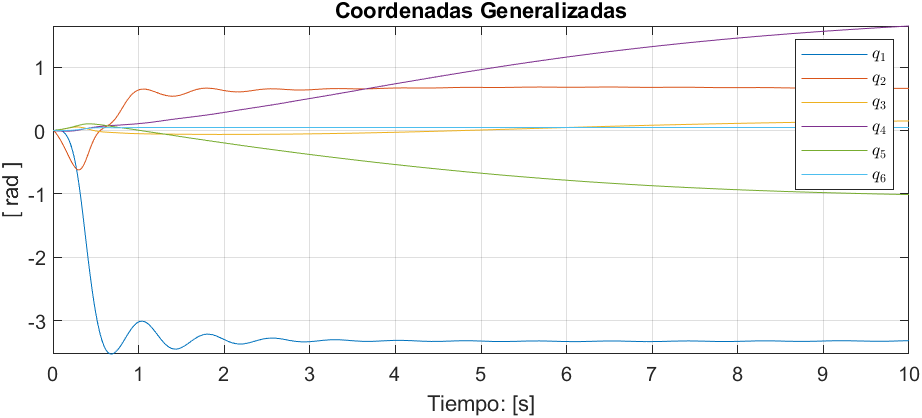
\includegraphics[scale=0.5]{coor_gen_caso_1.png} 
        \caption{Coordenadas Generalizadas Caso 1}
        \label{fig:CoordGenC1}
    \end{figure}

    \subsubsection{Velocidades Generalizadas}
    \noindent La gráfica \ref{fig:VelGenC1}, presenta un cambio notable en la velocidad 
    de las articulaciones $q_1$ y $q_2$, esto debido a que ambas conforman 
    las articulaciones base del robot, y por lo tanto permiten definir la dirección 
    de movimiento del resto de los referenciales. De esta forma se explican las 
    variaciones de velocidad significativas de las primeras dos articulaciones, 
    mientras que el resto, cuyos eslabones se mueven en función de los dos primeros 
    en una respuesta libre del sistema, muestran variaciones menores de velocidad.

    \begin{figure}[H]% [!ht]
            \centering
            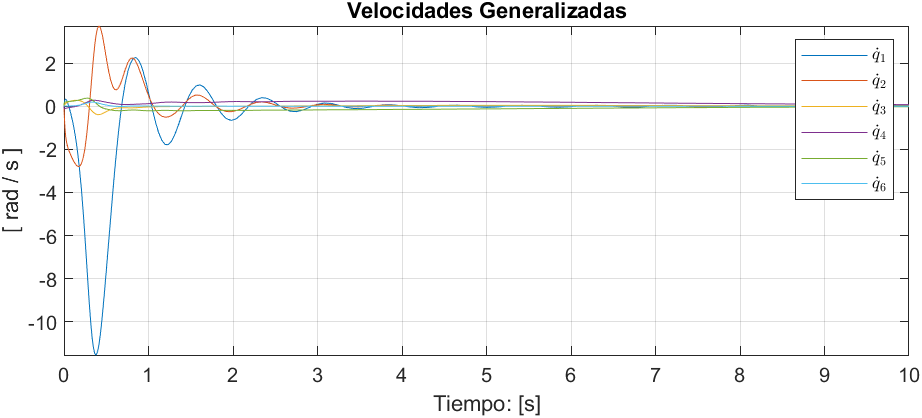
\includegraphics[scale=0.5]{vel_gen_caso_1.png} 
        \caption{Velocidad Generalizada Caso 1}
        \label{fig:VelGenC1}
    \end{figure}

    \subsubsection{Energía Cinética}
    \noindent En el caso de la figura \ref{fig:eCinC1} se observa un pico en la energía 
    cinética a los $0.4$ $[s]$ y un punto de inflexión hacia un estado estacionario 
    a partir de $2$ $[s]$, lo cual 
    es consistente con lo esperado, puesto que se observa una etapa de 
    amortiguamiento y pérdida de energía, hasta alcanzar el equilibrio. 
    
    Esto significa 
    que cuando se suelta el exoesqueleto de su posición de \emph{casa} y 
    empiece a moverse como un péndulo, llegará un instante en que se detenga el 
    movimiento oscilatorio, que es la fase de amortiguamiento observada.

    \begin{figure}[H]%[!ht]
            \centering
            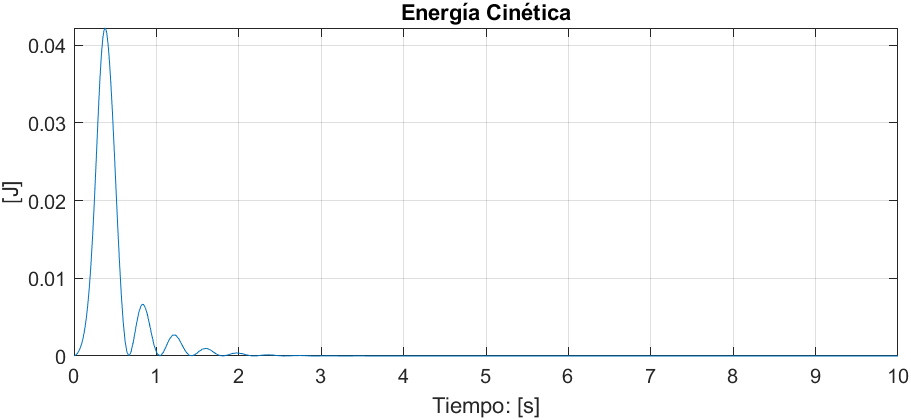
\includegraphics[scale=0.5]{ener_cin_caso_1.png} 
        \caption{Energía Cinética Caso 1}
        \label{fig:eCinC1}
    \end{figure}

    \subsubsection{Energía Potencial}
    \noindent La energía potencial inicia en $0.3$ $[J]$ y se puede observar en la Figura 
    \ref{fig:ePotC1} que a partir de $2$ $[s]$ se llega a un punto de equilibrio al no tener 
    movimiento el exoesqueleto. Esto es consistente con los resultados obtenidos para 
    el rango máximo de la energía cinética, pues la misma no adquiere valores mayores al 
    inicial de la energía potencial, con lo cual se demuestra el efecto directo de las 
    fuerzas disipativas.

    \begin{figure} [H]%[!ht]
            \centering
            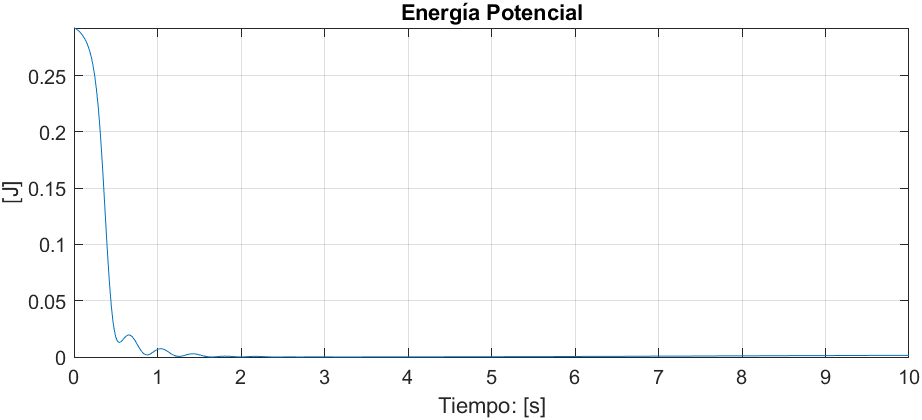
\includegraphics[scale=0.5]{ener_pot_caso_1.png} 
        \caption{Energía Potencial Caso 1}
        \label{fig:ePotC1}
    \end{figure}

    \subsubsection{Energía Mecánica}
    \noindent La gráfica de la Figura \ref{fig:eMecC1} resulta similar a la obtenida en la Figura \ref{fig:ePotC1} 
    debido a que la energía cinética presenta valores de una escala menor que los 
    obtenidos por la energía potencial, siendo congruente con que el cambio de la energía
    mecánica dependa principalmente de $\boldsymbol{U}$.

    \begin{figure} [H]%[!ht]
            \centering
            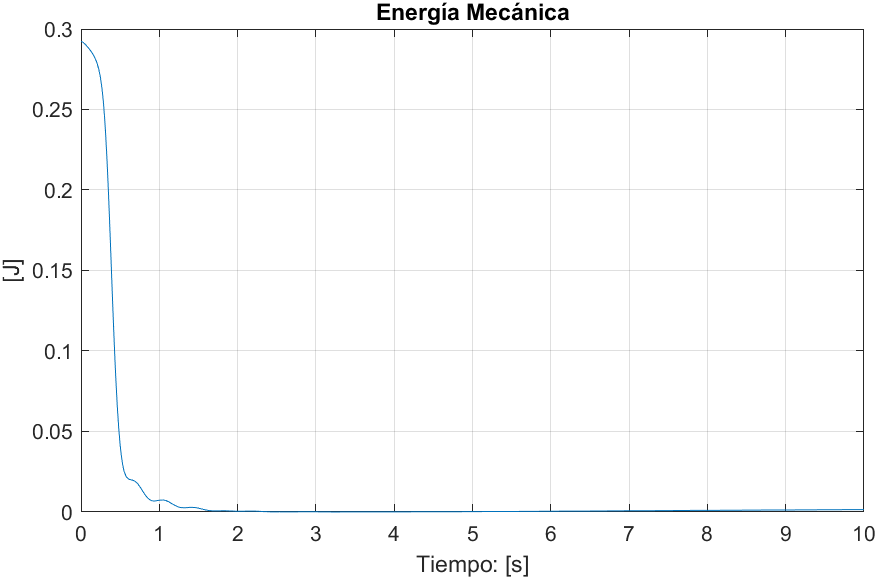
\includegraphics[scale=0.5]{ener_mec_caso_1.png} 
        \caption{Energía Mecánica Caso 1}
        \label{fig:eMecC1}
    \end{figure}

\subsection{Caso 2}\label{caso2}
    \noindent En el presente caso de estudio, se hicieron modificaciones en todos los 
    parámetros de acuerdo a los valores del Cuadro \ref{ref:TablaC2} para un 
    \textbf{sistema no conservativo} ante una respuesta a la entrada $\boldsymbol{\tau}$.

    \subsubsection{Parámetros} 
    \begin{table}[H]%[!ht]
        \centering
        \begin{center}
        \caption{Parámetros modificados del simulador} 
        \centering
        \scalebox{0.7}{
            \begin{tabular}{c||cccccc|c}
            Parámetros & $\tau_1$ & $\tau_2$ & $\tau_3$ & $\tau_4$ & $\tau_5$ & $\tau_6$ & Unidades\\
            \hline
            Torques & -0.050 & 0.050 & -0.040 & -0.060 & 0.020 & 0.010 & [Nm] \\
            Factor de Disipación & \multicolumn{6}{c|}{0.006001} & [Ns/m] \\
            Tiempo de Simulación & \multicolumn{6}{c|}{20} & [s]\\
            \hline 
            \end{tabular}    }
        \end{center}
        \label{ref:TablaC2}
    \end{table}

    \subsubsection{Coordenadas Generalizadas}
    \noindent Los resultados de la Figura \ref{fig:CoordGenC2} son consistentes con los 
    valores dados en los torques, considerando que las fuerza aplicadas en las 
    articulaciones $q_1$, $q_3$ y $q_4$ se definieron con valores negativos,
    representado un giro en sentido negativo acorde a la regla 
    de la mano derecha.

    \begin{figure} [H]%[!ht]
            \centering
            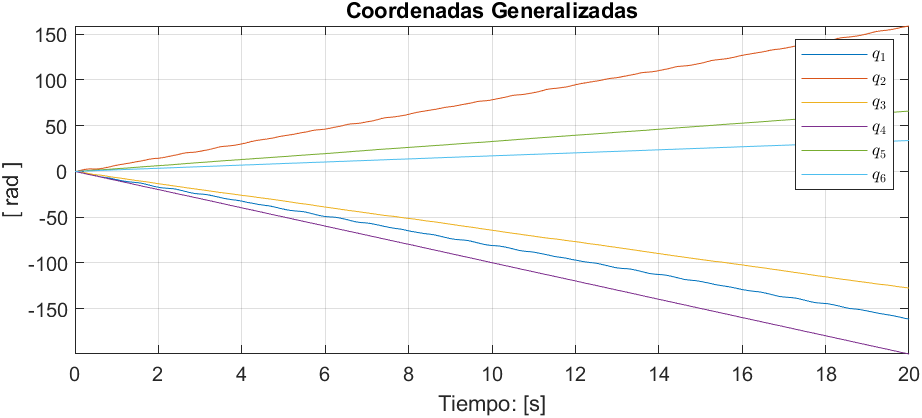
\includegraphics[scale=0.5]{coor_gen_caso_2.png} 
        \caption{Coordenadas Generalizadas Caso 2}
        \label{fig:CoordGenC2}
    \end{figure}

    \subsubsection{Velocidad Generalizada}
    \noindent Las articulaciones $q_1$ y $q_2$, en la Figura \ref{fig:VelGenC2}, 
    son las que presentan mayores variaciones de velocidad.
    Además, se considera que las velocidades $\dot{q}_2$, $\dot{q}_5$ y 
    $\dot{q}_6$ toman valores positivos de acuerdo a los torques aplicados.
    \begin{figure}[H]%[!ht]
            \centering
            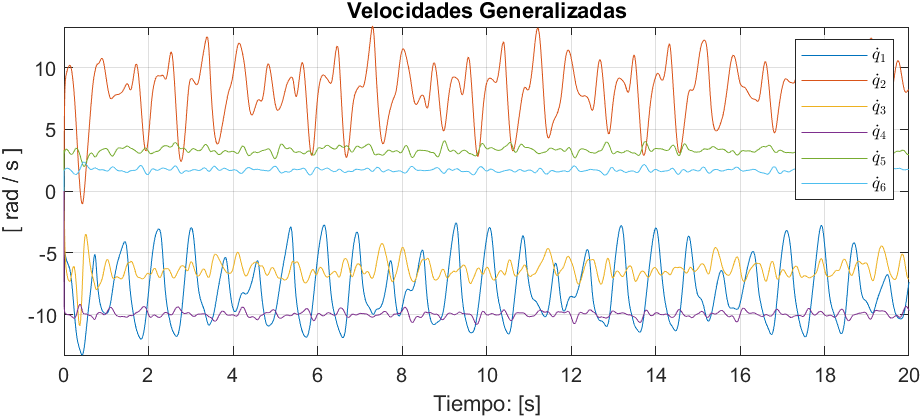
\includegraphics[scale=0.5]{vel_gen_caso_2.png} 
        \caption{Velocidad Generalizada Caso 2}
        \label{fig:VelGenC2}
    \end{figure}

    \subsubsection{Energía Cinética}
    \noindent La Figura \ref{fig:eCinC2} demuestra una función oscilatoria, la cual presenta valores 
    consistentes con el fenómeno físico que se observaría en el exoesqueleto al momento de 
    aplicar torques constantes. Ya que a diferencia del caso anterior en el que se presentaba 
    un punto de equilibrio, ahora las articulaciones se encuentran rotando de manera 
    permanente, ocasionando cambios en su energía cinética siempre que los torque sean mayores que 
    la energía potencial gravitacional.

    \begin{figure} [H]%[!ht]
            \centering
            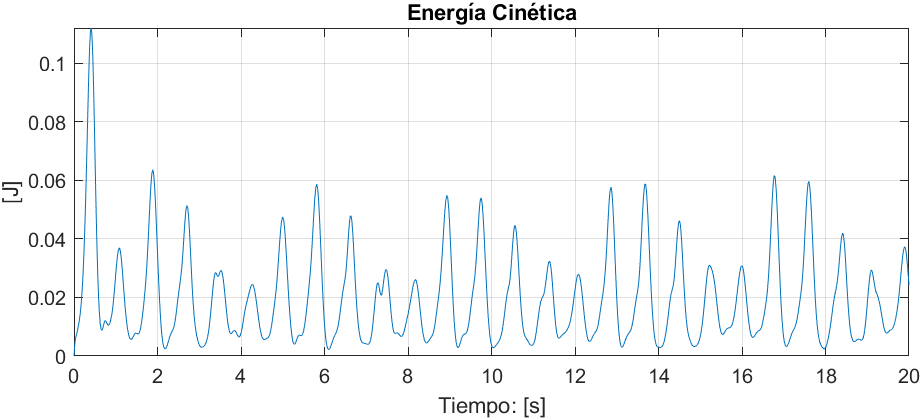
\includegraphics[scale=0.5]{ener_cin_caso_2.png} 
        \caption{Energía Cinética Caso 2}
        \label{fig:eCinC2}
    \end{figure}

    \subsubsection{Energía Potencial}
    Del mismo modo, la Figura 
    \ref{fig:ePotC2}  muestra la oscilación del movimiento que está teniendo 
    el exoesqueleto con valores energéticos entre $0$ $[J]$ y $2.2$ $[J]$
    sin alcanzar los $3$ $[J]$ del inicio, dado que el sistema no vuelve a tener la pose inicial. 
    
    Asimismo, se observa que los puntos de energía potencial máxima se relacionan con 
    los incrementos de energía cinética tanto por los efectos de la fuerza de gravedad como de las 
    exógenas aplicadas en cada GdL. 

    \begin{figure} [H]%[!ht]
            \centering
            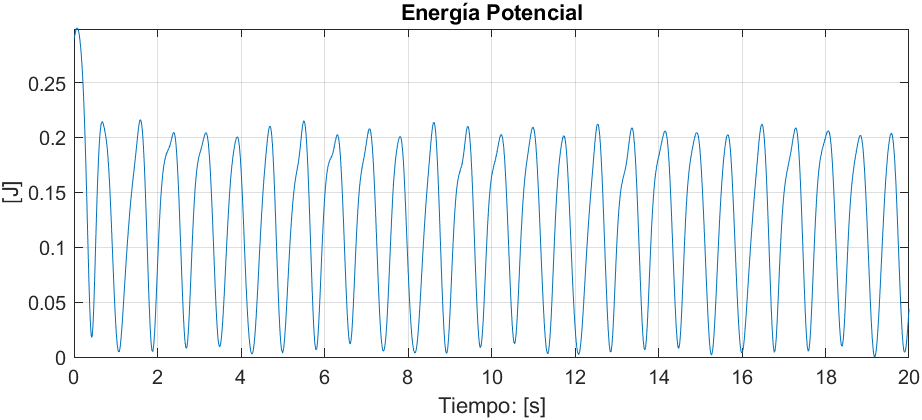
\includegraphics[scale=0.5]{ener_pot_caso_2.png} 
        \caption{Energía Potencial Caso 2}
        \label{fig:ePotC2}
    \end{figure}

    \subsubsection{Energía Mecánica}
    \noindent La Figura \ref{fig:eMecC2} muestra un desfase positivo, 
    proporcional a la magnitud de la energía cinética respecto a la 
    gráfica de la Figura \ref{fig:ePotC2}.
    \begin{figure} [H]%[!ht]
            \centering
            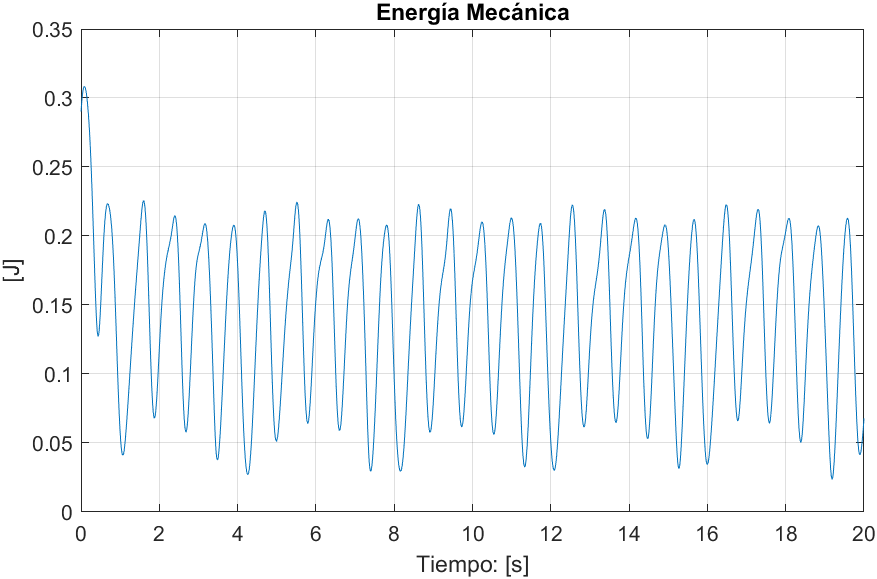
\includegraphics[scale=0.5]{ener_mec_caso_2.png} 
        \caption{Energía Mecánica Caso 2}
        \label{fig:eMecC2}
    \end{figure}

    

\subsection{Caso 3}\label{caso3}
    \noindent El último caso analizado representa un \textbf{sistema conservativo}, esto significa 
    un acercamiento a un sistema ideal o aislado, donde no se consideran fuerzas exógenas
    ni de disipación. En partícular, toda la energía mecánica del sistema es proporcional
    a la energía potencial máxima en la posición inicial. 

    \subsubsection{Parámetros}
    \noindent Los parámetros que se utilizaron para el caso 3, se ven reflejados en el 
    Cuadro \ref{ref:TablaC3}. Se incrementó el tiempo de simulación, para tener un 
    mayor tiempo de muestreo en el análisis.

    \begin{table}[H]%[!ht]
        \centering
        \begin{center}
        \caption{Parámetros modificados del simulador (Sistema Conservativo)} 
        \centering
        \scalebox{0.7}{
            \begin{tabular}{c||cccccc|c}
            Parámetros & $\tau_1$ & $\tau_2$ & $\tau_3$ & $\tau_4$ & $\tau_5$ & $\tau_6$ & Unidades\\
            \hline
            Torques & 0 & 0 & 0 & 0 & 0 & 0 & [Nm] \\
            Factor de Disipación & \multicolumn{6}{c|}{0} & [Ns/m] \\
            Tiempo de Simulación & \multicolumn{6}{c|}{200} & [s]\\
            \hline 
            \end{tabular}    }
        \end{center}
        \label{ref:TablaC3}
    \end{table}

    \subsubsection{Coordenadas Generalizadas}
    \noindent La gráfica de la Figura \ref{fig:CoordGenC3} muestra los cambios en la posición 
    angular de cada una de las articulaciones a lo largo de $200$ $[s]$. 
    Se aprecia $q_6$ ejecuta mayor número de rotaciones. 

    \begin{figure} [H]% [!ht]
            \centering
            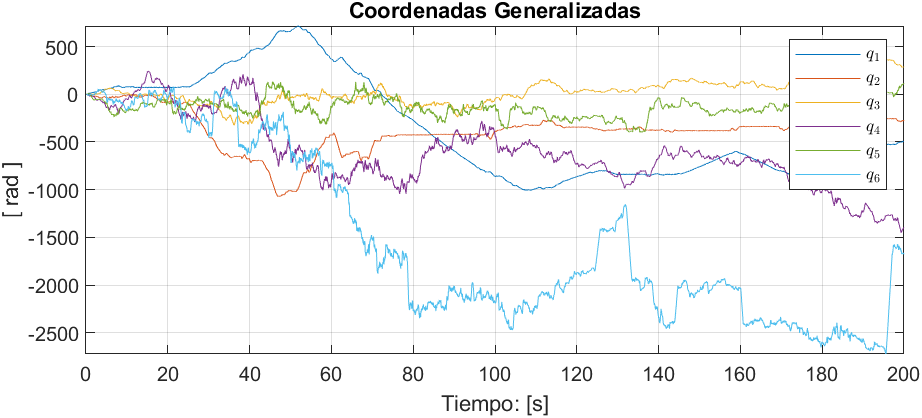
\includegraphics[scale=0.5]{coor_gen_caso_3.png} 
        \caption{Coordenadas Generalizadas Caso 3}
        \label{fig:CoordGenC3}
    \end{figure}

    \subsubsection{Velocidad Generalizada}
    \noindent Por otro lado, la Figura \ref{fig:VelGenC3} muestra en primer plano la velocidad 
    generalizada del referencial $q_6$ en azul claro. El cual, entre $0$ a $40$ $[s]$
    presenta un incremento positivo en sus valores 
    de velocidad, alcanzando su punto máximo en $68$ $[s]$. Posteriormente,
    empieza a disminuir su velocidad hasta alcanzar un rango de $-1000$ a $1000$ 
    $[rad/s]$ a partir de un tiempo de 120 segundos. 

    \begin{figure}[H]%[!ht]
            \centering
            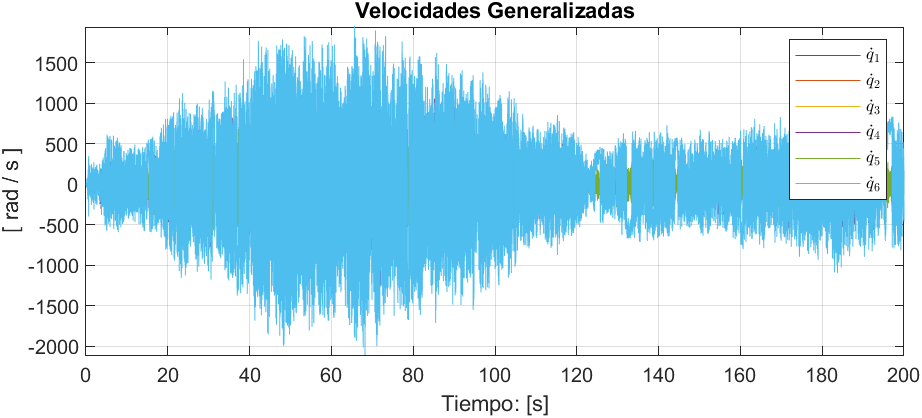
\includegraphics[scale=0.5]{vel_gen_caso_3.png} 
        \caption{Velocidad Generalizada Caso 3}
        \label{fig:VelGenC3}
    \end{figure}

    \subsubsection{Energía Cinética}
    \noindent La energía cinética representada en la Figura \ref{fig:eCinC3} muestra 
    un pico en $68$ $[s]$. Posteriormente, alcanza rango definido entre 
    $0$ y $1$ $[J]$ a partir de $120$ $[s]$ similar al comportamiento de $\dot{q}_6$.

    \begin{figure} [H]%[!ht]
            \centering
            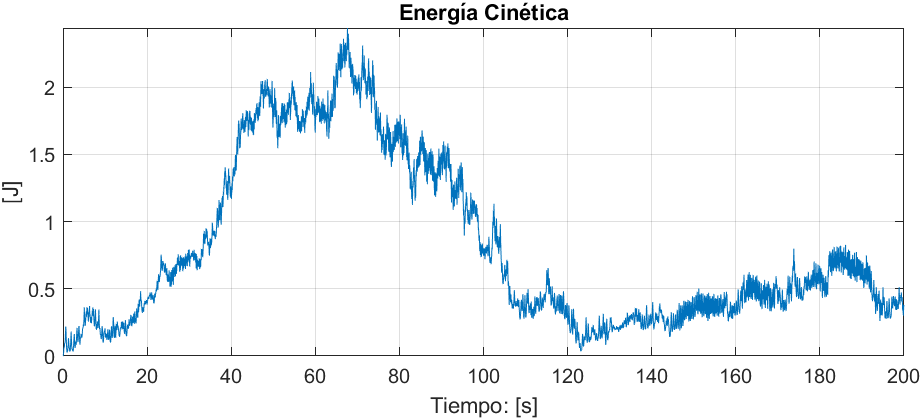
\includegraphics[scale=0.5]{ener_cin_caso_3.png} 
        \caption{Energía Cinética Caso 3}
        \label{fig:eCinC3}
    \end{figure}

    \subsubsection{Energía Potencial}
    \noindent Considerando el ajuste del \emph{datum} de la Energía Potencial de acuerdo a (\ref{eqn:energia_potencial_offset}),
    los valores presentes en la Figura \ref{fig:ePotC3} se definen en un rango entre $0$ y 
    $0.3$ $[J]$.

    \begin{figure} [H]%[!ht]
            \centering
            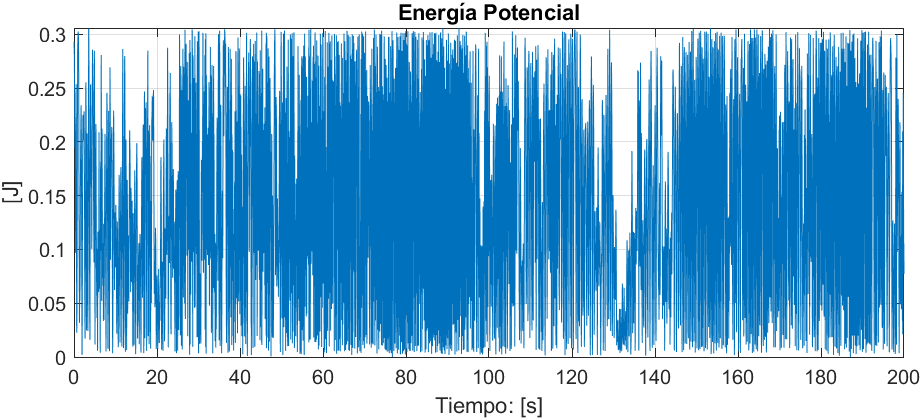
\includegraphics[scale=0.5]{ener_pot_caso_3.png} 
        \caption{Energía Potencial Caso 3}
        \label{fig:ePotC3}
    \end{figure}

    \subsubsection{Energía Mecánica}
    \noindent La Figura \ref{fig:eMecC3} representa la energía mecánica total de 
    un sistema conservativo cuyo valor máximo es $0.3$ $[J]$ proporcional a
    la energía potencial en la posición inicial. 

    Sin embargo, se observa que entre $0$ a $68$ $[s]$ se refleja una inconsistencia
    a las \emph{leyes de la termodinámica} al ir en aumento la energía cinética y 
    superar el rango máximo de la energía potencial.

    \begin{figure}[H]%[!ht]
            \centering
            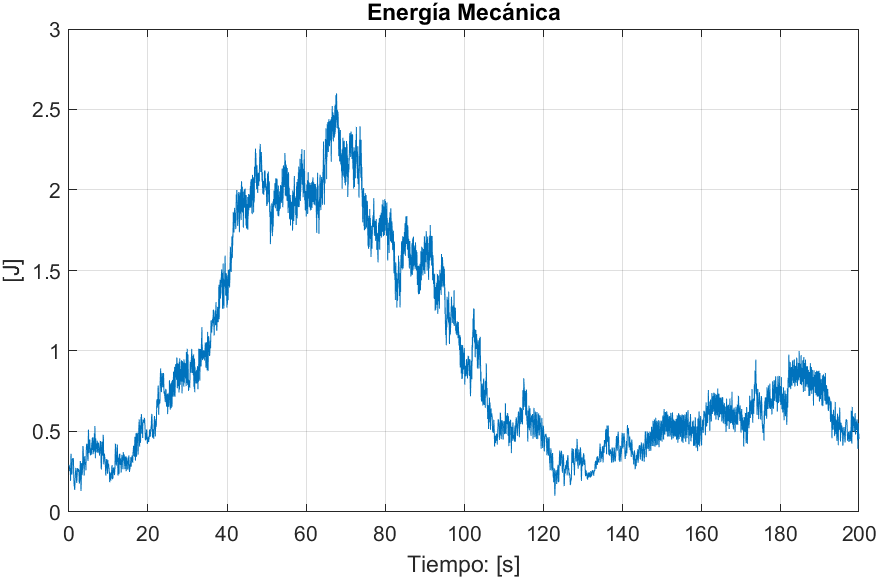
\includegraphics[scale=0.5]{ener_mec_caso_3.png} 
        \caption{Energía Mecánica Caso 3}
        \label{fig:eMecC3}
    \end{figure}